\chapter{逆时偏移算法}\label{chap:RTM}

\section{数值算例}
\section{散射系数与 Kirchhoff 逼近}

\subsection{反射面为$x_1$轴}

We consider the scattering of an incident plane $p$-wave  $\hat u_p$ (or $s$-wave $\hat u_s$) with the incident direction $\hat d_0=(\sin t_0, \cos t_0)^T, t_0\in (0,2\pi)$, by the plane $\Gamma := \{x \in \R^2 :x _2 = 0\}$. 
The angle between $\hat d_0$ and the positive real axis is $\theta_0=\pi/2-t_0$. Denote by $\hat\nu=(0,1)^T$.

\subsubsection{$p$-波情形}
We denote the incident $p$-wave \cite[p172]{achenbach1980} as
\ben
\hat u_p=A_0(\sin t_0,\cos t_0)^Te^{\i k_p(x_1\sin t_0+x_2 \cos t_0)}.
\een
The reflected $p$-wave is represented as
\ben
\hat u_{p,p}=A_1(\sin t_1,-\cos t_1)^Te^{\i k_p(x_1\sin t_1-x_2 \cos t_1)}.
\een
The reflected $s$-wave is denoted as
\ben
& &\hat u_{p,s}=A_2(-\cos t_2,-\sin t_2)^Te^{\i k_s(x_1\sin t_2-x_2 \cos t_2)}.
\een
Under the clamped condition, the total field vanishes on $\Ga$ and thus
\ben
\hat u_p(x_1,0)+\hat u_{p,p}(x_1,0)+\hat u_{p,s}(x_1,0)=0,\ \ \forall x_1\in\R.
\een
A simple computation shows that
\ben
t_1=t_0, \ \ \frac{\sin t_2}{\sin t_0}=\frac{k_p}{k_s}:=\kappa, \\
A_0=\cos(t_0-t_2), \ \ A_1=\cos(t_0+t_2), \ \ A_2=\sin 2t_0.
\een
In summary, the total field is
\be\label{a1}
\hat u^{\rm total}_p=A_0\hat d_0e^{\i k_px\cdot\hat d_0}+A_1\hat d_1e^{\i k_px\cdot\hat d_1}+A_2\hat d_2^\perp e^{\i k_s x\cdot\hat d_2},
\ee
where for any $\tau=(\tau_1,\tau_2)^T\in\R^2$, $\tau^\perp=(\tau_2,-\tau_1)^T$, and
\be
\hskip-2cm& &\hat d_1=\hat d_0-2(\hat d_0\cdot\hat\nu)\hat\nu, \hat d_2=\kappa\hat d_0-\left[\kappa(\hat d_0\cdot\hat\nu)+{\rm sgn}(\hat d_0\cdot\hat\nu)\sqrt{1-\kappa^2(\hat d_0\cdot\hat\nu^\perp)^2}\,\right]\hat\nu,\\
\hskip-2cm& &A_0=\hat d_1\cdot\hat d_2, A_1=-\hat d_0\cdot\hat d_2,A_2=2(\hat d_0\cdot\hat\nu)(\hat d_0\cdot\hat\nu^\perp).\label{a2}
\ee

\subsubsection{$s$-波情形}
We denote the incident $s$-wave as 
\ben
& &\hat u_s=A_0(\cos t_0,-\sin t_0)^Te^{\i k_s(x_1\sin t_0+x_2 \cos t_0)}.
\een
The reflected $p$-wave is represented as
\ben
\hat u_{s,p}=A_1(\sin t_1,-\cos t_1)^Te^{\i k_p(x_1\sin t_1-x_2 \cos t_1)}.
\een
The reflected $s$-wave is denoted as
\ben
& &\hat u_{s,s}=A_2(-\cos t_2,-\sin t_2)^Te^{\i k_s(x_1\sin t_2-x_2 \cos t_2)}.
\een
The result is 
\ben
t_2=t_0,\ \ \frac{\sin t_1}{\sin t_0}=\frac{k_s}{k_p}=\kappa_1,\\
A_0=\cos(t_0-t_1),\ \ A_1=-\sin 2t_0,\ \ A_2=\cos(t_0+t_1).
\een
In summary, the total field is
\be\label{b1}
\hat u^{\rm total}_s=A_0\hat d_0^\perp e^{\i k_sx\cdot\hat d_0}+A_1\hat d_1e^{\i k_px\cdot\hat d_1}+A_2\hat d_2^\perp e^{\i k_s x\cdot\hat d_2},
\ee
where 
\be
\hskip-2cm& &\hat d_1=\kappa_1\hat d_0-\left[\kappa_1(\hat d_0\cdot\hat\nu)+{\rm sgn}(\hat d_0\cdot\hat\nu)\sqrt{1-\kappa_1^2(\hat d_0\cdot\hat\nu^\perp)^2}\,\right]\hat\nu, \hat d_2=\hat d_0-2(\hat d_0\cdot\hat\nu)\hat\nu,\\
\hskip-2cm& &A_0=\hat d_1\cdot\hat d_2, A_1=-2(\hat d_0\cdot\hat\nu)(\hat d_0\cdot\hat\nu^\perp),A_2=-\hat d_0\cdot\hat d_1.\label{b2}
\ee

\subsection{反射面为任意平面}

We consider the scattering of an incident plane $p$-wave  $u_p$ or $s$-wave $u_s$ with the incident direction $d=(\sin\theta,\cos\theta)^T,\theta\in (0,2\pi)$, by the plane $\Gamma := \{x \in \R^2 : x \cdot \nu = 0\}$ through the origin with the normal vector $\nu=(\sin\phi,\cos\phi)^T,\phi\in (0,2\pi)$. The angle between $\nu$ and the positive real axis is $\pi/2-\phi$. The total fields are
\be
u_p^{\rm total}=A_0d_0 e^{\i k_p x\cdot d_0}+A_1 d_1 e^{\i k_p x\cdot d_1}+A _2d_2^\perp e^{\i k_s x\cdot d_2},\\
u_s^{\rm total}=A_0d_0^\perp e^{\i k_s x\cdot d_0}+A_1 d_1 e^{\i k_p x\cdot d_1}+A_2 d_2^\perp e^{\i k_s x\cdot d_2},
\ee
where for $i=0,1,2$, $d_i$ is the unit vector and $A_i$ is the corresponding amplitude. We impose $u_p^{\rm total}=0, u_s^{\rm total}=0$ on $\Gamma$. Let  
$\hat x= S x$, where $S\in\R^{2\times 2}$ is the rotation matrix with rotation angle $\phi$,
\ben
S= \left( \begin{array}{ll}
	\cos\phi& -\sin\phi \\
	\sin\phi & \cos\phi
\end{array}\right).
\een
We have $\hat\nu=S\nu$.

\begin{thm}
	Let $u(x)\in \C^2$ and
	\ben
	\Delta_e^x := \left(\begin{array}{ll}
		(\lambda +2\mu)\frac{\pa^2 }{\pa x_1^2}+(\lambda +\mu) \frac{\pa^2}{\pa x_1\pa x_2} +\mu \frac{\pa^2}{\pa x_2^2}\\
		\mu \frac{\pa^2}{\pa x_1^2}+(\lambda +\mu) \frac{\pa^2}{\pa x_1\pa x_2}+(\lambda +2\mu)\frac{\pa^2 }{\pa x_12^2}
	\end{array}\right).
	\een
	Assume that u(x) satisfies $\Delta_e^x u(x)+\omega^2 u(x)=0$, then  we have $\Delta_e^{\hat x} \hat u(\hat x)+\omega^2 \hat u(\hat x)=0$ where $\hat u(\hat x):= S u(S^T\hat x)$ or $u(x)=S^T\hat u(Sx)$.
\end{thm}

\debproof
Since
\ben
\frac{\pa^2}{\pa \hat x_1^2}=\cos^2\phi \frac{\pa^2}{\pa  x_1^2}-2\cos\phi\sin\phi \frac{\pa^2}{\pa  x_1\pa x_2}+\sin^2\phi \frac{\pa^2}{\pa  x_2^2} \\
\frac{\pa^2}{\pa \hat x_2^2}=\sin^2\phi \frac{\pa^2}{\pa  x_1^2}+2\cos\phi\sin\phi \frac{\pa^2}{\pa  x_1\pa x_2}+\cos^2\phi \frac{\pa^2}{\pa  x_2^2} \\
\frac{\pa^2}{\pa \hat x_1 \pa\hat x_2}=\cos\phi\sin\phi\frac{\pa^2}{\pa  x_1^2}+(\cos^2\phi-\sin^2\phi) \frac{\pa^2}{\pa  x_1\pa x_2}-\cos\phi\sin\phi\frac{\pa^2}{\pa  x_2^2}
\een
This completes proof after substituting above equation into $\Delta_e^{\hat x} \hat u(\hat x)$.
\finproof

By this theorem, we obtain from (\ref{a1})-(\ref{a2}) that for $u_p^{\rm total}$, $d_0=(\sin(\theta-\phi),\cos(\theta-\phi))^T$,
\ben
\hskip-2cm& &d_1=d_0-2(d_0\cdot\nu)\nu,d_2=\kappa d_0-\left[\kappa(d_0\cdot\nu)+{\rm sgn}(d_0\cdot\nu)\sqrt{1-\kappa^2(d_0\cdot\nu^\perp)^2}\,\right]\nu, \\
\hskip-2cm& &A_0=d_1\cdot d_2, A_1=-d_0\cdot d_2,A_2=2(d_0\cdot\nu)(d_0\cdot\nu^\perp).
\een
In fact, we have

\ben
u^{\rm total}_p(x)&=&S^T\hat u_p^{\rm total}(Sx)\\
&=&S^T\left[A_0\hat d_0e^{\i k_pSx\cdot\hat d_0}+A_1\hat d_1e^{\i k_pSx\cdot\hat d_1}+A_2\hat d_2^\perp e^{\i k_s Sx\cdot\hat d_2}\right].
\een
This implies $S^T\hat d_j=d_j$, $j=0,1,2$. As $d_0=d$, we obtain $\hat d_0=Sd$.
Similarly, for $u_s^{\rm total}$,  $d_0=(\sin(\theta-\phi),\cos(\theta-\phi))^T$,
\ben
\hskip-2cm& &d_1=\kappa_1 d_0-\left[\kappa_1(d_0\cdot\nu)+{\rm sgn}(d_0\cdot\nu)\sqrt{1-\kappa_1^2(d_0\cdot\nu^\perp)^2}\,\right]\nu, d_2=d_0-2(d_0\cdot\nu)\nu,\\
\hskip-2cm& &A_0=d_1\cdot d_2, A_1=-2(d_0\cdot\nu)(d_0\cdot\nu^\perp),A_2=-d_0\cdot d_1.
\een
The traction of $u(x)$ on the plane $\Gamma$ can be obtained by simple calculation
\be
\sigma(u_p^{\rm total})\cdot\nu&=&[\i k_p A_0 (\lambda\nu+2\mu(d_0,\nu)d_0)+\i k_p A_1 (\lambda\nu+2\mu(d_1,\nu)d_1)\nn\\
& &+\i k_s A_2\mu((d_2,\nu)d_2^\perp+(d_2^\perp,\nu)d_2)]e^{\i k_p x\cdot d_0}\nn\\
&:=&\i k_p A_0 \hat{\mathbf{R}}_p(x,d_0,\nu) e^{\i k_p x\cdot d_0},\label{kir_p}\\
\sigma(u_s^{\rm total})\cdot\nu&=&[\i k_s A_0 \mu((d_0,\nu)d_0^\perp+(d_0^\perp,\nu)d_0)+\i k_p A_1 (\lambda\nu+2\mu(d_1,\nu)d_1)\nn\\
& &+\i k_s A_2\mu((d_2,\nu)d_2^\perp+(d_2^\perp,\nu)d_2)]e^{\i k_s x\cdot d_0}\nn\\
&:=&\i k_s A_0\hat {\mathbf{R}}_s(x,d_0,\nu) e^{\i k_s x\cdot d_0}.\label{kir_s}
\ee


\begin{definition}
	For any unit vector $d\in \R^2$, let $u^i_p =d e^{\i k_p x\cdot d}$ or $u^i_s= d^\perp e^{\i k_s x\cdot d}$ be the incident wave and $u^s_\alpha = u^s_\alpha(x;d)$ be the radiation solution of the Navier equation:
	\ben
	u^s_\alpha + \om^2u^s_\alpha = 0\ \ \mbox{in} \ \  \R^2\bks\bar{D} \\
	\Delta_e	u^s_\alpha =-u^i_\alpha \ \ \mbox{on} \ \ \pa D 
	\een
	The scattering coefficient $\mathbf{R}_\alpha(x;d)$ for $x\in\pa D$ is defined by the relation
	\ben
	\sigma(u^s_\alpha+u^i_\alpha)\cdot \nu= \i k_\alpha \mathbf{R}_\alpha(x;d)e^{\i k_\alpha x\cdot d}  \ \ \ \mbox{on}\ \ \pa D
	\een
	where $\alpha=p,s$.
\end{definition}

For a convex object $D$, Kirchhoff approximation approximates the scattering coefficient by considering 
the boundary at $x\in\pa D$ locally as a plane with normal $\nu$ to obtain
\ben
\mathbf{R}_\alpha(x;d)\approx\left\{ \begin{array}{ll}
	\hat {\mathbf{R}}_\alpha(x;d,\nu(x))    \ \  \  \mbox{if} \ \ x \in \pa D^{-}_d=\{x\in \pa D, \nu(x)\cdot d<0\},\\ 
	0 \ \ \ \ \ \ \ \  \ \ \ \ \ \ \ \ \mbox{if} \ \ x \in \pa D^{+}_d=\{x\in \pa D, \nu(x)\cdot d\geq0\}.
\end{array} \right.
\een


\subsection{数值算例}
In this section we present several numerical examples to show the effectiveness of Kirchhoff approximation. To synthesize the real scattering coefficient we compute the solution $\sigma(u^s_\alpha+u^i_\alpha)\cdot \nu$ of
the scattering problems by representing the ansatz solution as the single layer potential
with the Green tensor $\G(x,y)$ as the kernel
\ben\hspace{-2cm}
u^s(x)=\int_{\Ga_D} - \G(y,x)^T\sigma(u^s(y)+u^i(y))\nu ds(y)=-u^i(x) \ \ \ \  \mbox{on} \ \ x\in \Ga_D,
\een 
and discretizing the integral equation by
standard Nystr\"{o}m methods \cite{colton-kress}. Let $\mathbf{R}_\alpha(x;d)=(\mathbf{R}_\alpha^1(x;d),\mathbf{R}_\alpha^2(x;d))^T$, then we have
\be
\mathbf{R}_\alpha^j(x;d)=\frac{\sigma(u^s(y)+u^i(y))\nu\cdot e_j}{\i k_\alpha e^{\i k_\alpha x\cdot d} }.
\ee
We compute $\hat {\mathbf{R}}_\alpha(x;d)=(\hat {\mathbf{R}}_\alpha^1(x;d),\hat {\mathbf{R}}_\alpha^2(x;d))^T$ by (\ref{kir_p}) and (\ref{kir_s}).
In all our numerical examples we choose {Lam\'{e}} constant $\lambda=1/2$, $\mu=1/4$ and 
\ben
u^i_p=(\cos t,\sin t )^T e^{\i k_p(x_1 \cos t +x_2\sin t)} \\
u^i_s=(\sin t,-\cos t)^T e^{\i k_s(x_1 \cos t +x_2\sin t)}
\een where
$t\in[0,2\pi]$.. 
The boundaries
of the obstacles used in our numerical experiments are parameterized as follows:
\ben
\hskip-2cm\mbox{Circle:}\ \ \ \ x_1=\cos(\theta),\ \ x_2=\sin(\theta);\ \  \\
\hskip-2cm\mbox{Pear:}\ \ \ \rho = 0.5(2+0.3\cos(3\theta)),x_1=\sin \frac{\pi}{4}\rho(\cos\theta-\sin\theta),x_2=\sin \frac{\pi}{4}\rho(\cos\theta+\sin\theta),
\een
where

$\theta\in[0,2\pi]$ (See Figure \ref{shape}). 

In the following examples, we take the angular frequency $\omega= \pi,2\pi,4\pi,8\pi$.

\begin{figure}[htbp]
	\centering
	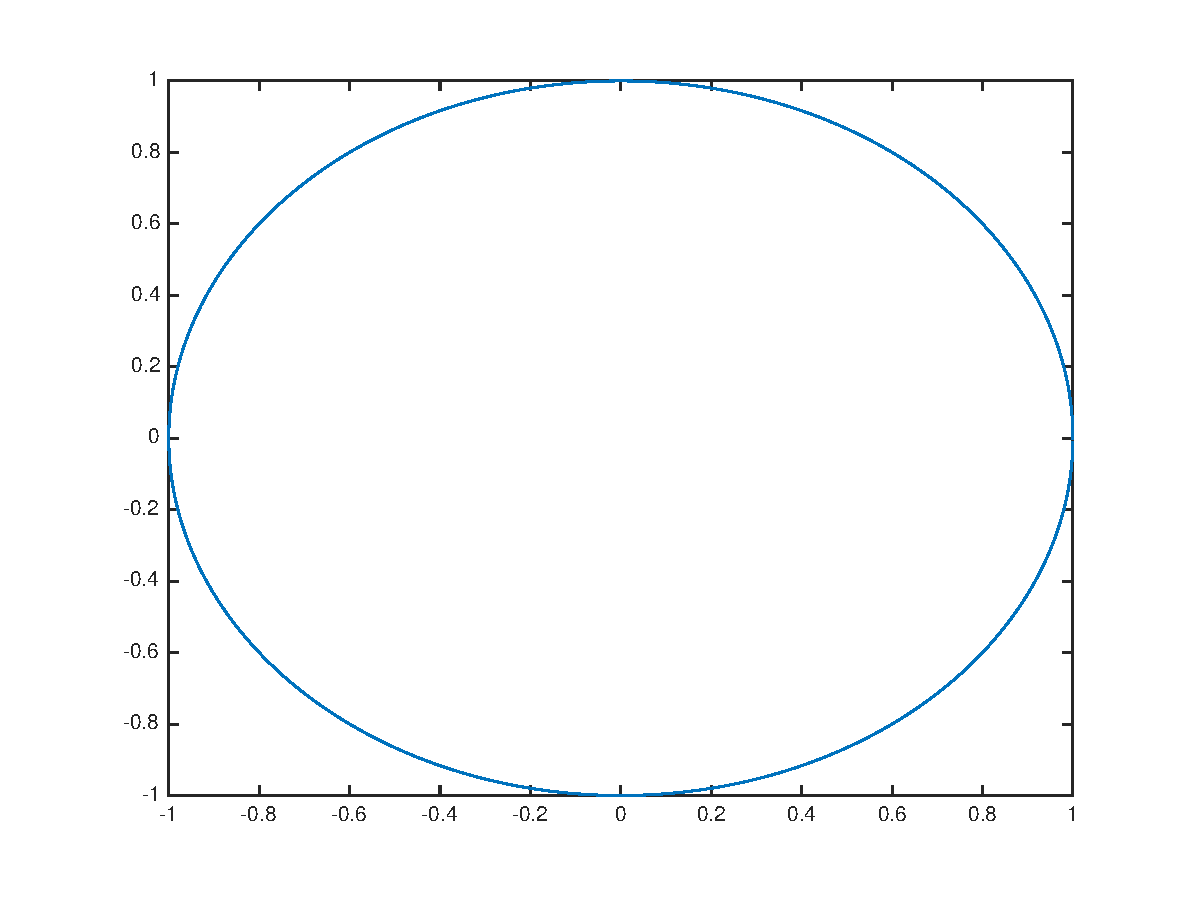
\includegraphics[width=0.48\textwidth]{./Img/figure_sc_elastic/circle.eps}
	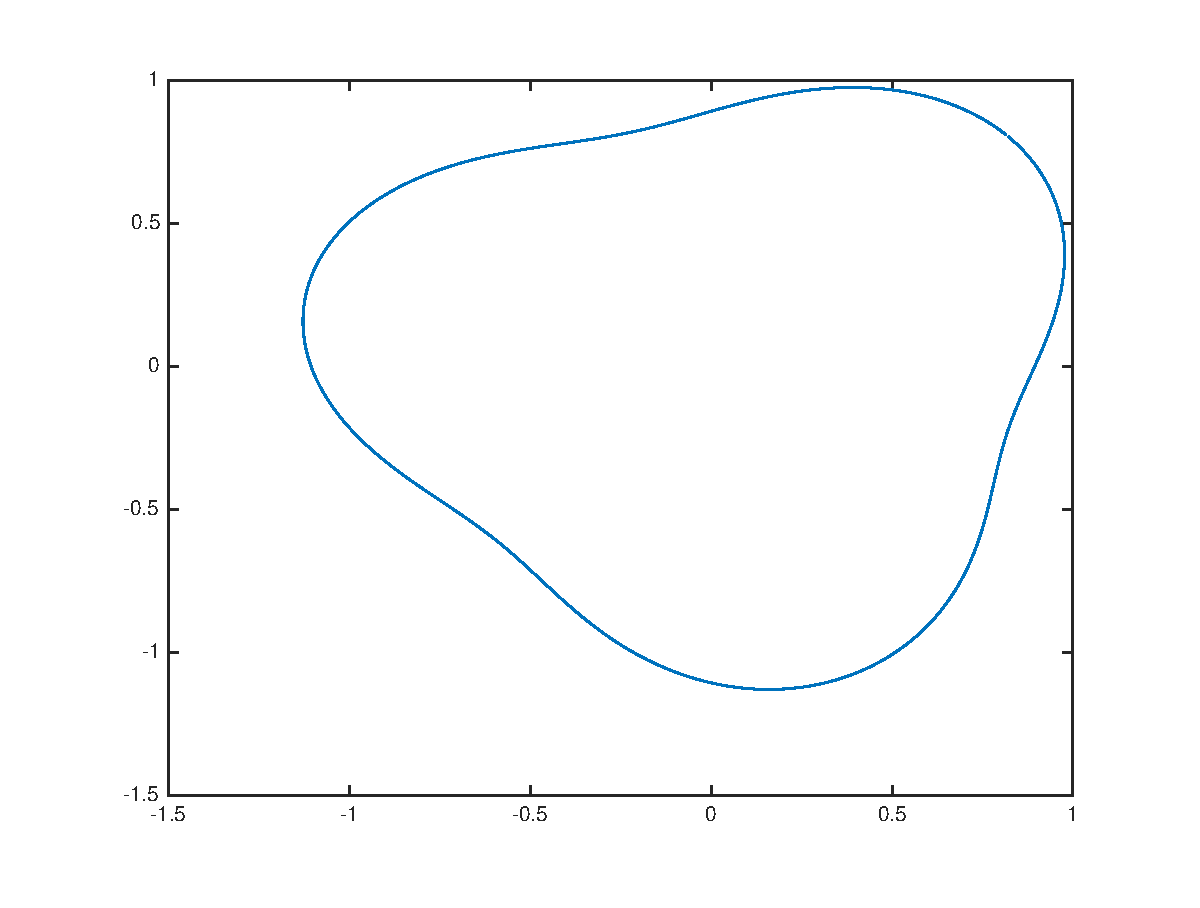
\includegraphics[width=0.48\textwidth]{./Img/figure_sc_elastic/pear.eps}
	\caption{The shape of the obstacles.}\label{shape}
\end{figure}




